%===============================================================================
%===============================================================================
%
\clearpage
%
\subsection{Example-0001}
%
Example uses generated regular meshes and solves a static problem, i.e., applies
the boundary conditions in one step.
%
%===============================================================================
%
\subsubsection{Mathematical model - 2D}
%
We solve the following scalar equation,
%
\begin{align}
    \nabla \cdot \nabla u = 0 & &&\Omega = [0, 2] \times [0, 1],
\end{align}
%
with boundary conditions
%
\begin{align}
    u = 0 & &&x = y = 0, \\
    u = 1 & &&x = 2, y = 1.
\end{align}
%
No material parameters to specify.
%
%===============================================================================
%
\subsubsection{Mathematical model - 3D}
%
We solve the following scalar equation,
%
\begin{align}
    \nabla \cdot \nabla u = 0 & &&\Omega = [0, 2] \times [0, 1] \times [0, 1],
\end{align}
%
with boundary conditions
%
\begin{align}
    u = 0 & &&x = y = z = 0, \\
    u = 1 & &&x = 2, y = z = 1.
\end{align}
%
No material parameters to specify.
%
%===============================================================================
%
\subsubsection{Computational model}
%
\begin{itemize}
    \item{Commandline arguments are:}
        \subitem{float: length along x-direction}
        \subitem{float: length along y-direction}
        \subitem{float: length along z-direction (set to zero for 2D)}
        \subitem{integer: number of elements in x-direction}
        \subitem{integer: number of elements in y-direction}
        \subitem{integer: number of elements in z-direction (set to zero for 2D)}
        \subitem{interger: interpolation order (1: linear; 2: quadratic)}
        \subitem{integer: solver type (0: direct; 1: iterative)}
    \item{Commandline arguments for tests are:}
        \subitem{2.0 1.0 0.0 2 1 0 1 0}
        \subitem{2.0 1.0 0.0 4 2 0 1 0}
        \subitem{2.0 1.0 0.0 8 4 0 1 0}
        \subitem{2.0 1.0 0.0 2 1 0 2 0}
        \subitem{2.0 1.0 0.0 4 2 0 2 0}
        \subitem{2.0 1.0 0.0 8 4 0 2 0}
        \subitem{2.0 1.0 0.0 2 1 0 1 1}
        \subitem{2.0 1.0 0.0 4 2 0 1 1}
        \subitem{2.0 1.0 0.0 8 4 0 1 1}
        \subitem{2.0 1.0 0.0 2 1 0 2 1}
        \subitem{2.0 1.0 0.0 4 2 0 2 1}
        \subitem{2.0 1.0 0.0 8 4 0 2 1}
        \subitem{2.0 1.0 1.0 2 1 1 1 0}
        \subitem{2.0 1.0 1.0 4 2 2 1 0}
        \subitem{2.0 1.0 1.0 8 4 4 1 0}
        \subitem{2.0 1.0 1.0 2 1 1 2 0}
        \subitem{2.0 1.0 1.0 4 2 2 2 0}
        \subitem{2.0 1.0 1.0 8 4 4 2 0}
        \subitem{2.0 1.0 1.0 2 1 1 1 1}
        \subitem{2.0 1.0 1.0 4 2 2 1 1}
        \subitem{2.0 1.0 1.0 8 4 4 1 1}
        \subitem{2.0 1.0 1.0 2 1 1 2 1}
        \subitem{2.0 1.0 1.0 4 2 2 2 1}
        \subitem{2.0 1.0 1.0 8 4 4 2 1}
\end{itemize}
%
%===============================================================================
%
\subsubsection{Result summary}
%
We use CHeart rev.\ 6292 to produce numerical reference solutions.
%
\verbatiminput{examples/example-0001/results/results.summary}
\verbatiminput{examples/example-0001/results/failed.tests}
%
%\begin{figure}[h!]
%    \centering 
%    \includegraphics[width=0.9\columnwidth]{examples/example-0001/doc/figures/analytical_solution.eps} 
%    \caption{Results, analytical solution.}
%    \label{example-0001-analytical-solution-fig}
%\end{figure}
%
%\begin{figure}[h!]
%    \centering 
%    \includegraphics[width=0.9\columnwidth]{examples/example-0001/doc/figures/abaqus_reference.eps} 
%    \caption{Results, Abaqus reference.}
%    \label{example-0001-abaqus-reference-fig}
%\end{figure}
%
\begin{figure}[h!]
    \centering 
    \includegraphics[width=0.9\columnwidth]{examples/example-0001/doc/figures/iron_reference_2D.eps} 
    \caption{2D results, iron reference w/ command line arguments [2.0 1.0 0.0 8 4 0 1 0].}
    \label{example-0001-iron-2D-reference-fig}
\end{figure}
%
\begin{figure}[h!]
    \centering 
    \includegraphics[width=0.9\columnwidth]{examples/example-0001/doc/figures/current_run_l2x1x0_n8x4x0_i1_s0.eps} 
    \caption{2D results, current run w/ command line arguments [2.0 1.0 0.0 8 4 0 1 0].}
    \label{example-0001-current-run-2D-fig}
\end{figure}
%
\begin{figure}[h!]
    \centering 
    \includegraphics[width=0.9\columnwidth]{examples/example-0001/doc/figures/iron_reference_3D.eps} 
    \caption{3D results, iron reference w/ command line arguments [2.0 1.0 1.0 8 4 4 1 0].}
    \label{example-0001-iron-3D-reference-fig}
\end{figure}
%
\begin{figure}[h!]
    \centering 
    \includegraphics[width=0.9\columnwidth]{examples/example-0001/doc/figures/current_run_l2x1x1_n8x4x4_i1_s0.eps} 
    \caption{3D results, current run w/ command line arguments [2.0 1.0 1.0 8 4 4 1 0].}
    \label{example-0001-current-run-3D-fig}
\end{figure}
%
%===============================================================================
%===============================================================================
